\hypertarget{programmeren}{%
\section{Programmeren}\label{programmeren}}

Nu we weten dat we gaan programmeren in de arduino-taal, de Nano
volledig naar toebehoren werkt en de juiste hardware binnen is, kunnen
we beginnen met programmeren. Hierin liepen we echter ook tegen
belangrijke keuzes en vele leermomenten aan. In deze paragraaf wordt
beschreven hoe dit proces te werk ging, en wat we daarvoor nodig hadden.

\hypertarget{ontwikkelingsomgeving}{%
\subsection{Ontwikkelingsomgeving}\label{ontwikkelingsomgeving}}

Wij hebben ervoor gekozen om de Arduino IDE niet te gebruiken in ons
ontwikkelproces. De IDE van Arduino mist vele functionaliteiten die het
ontwikkelen net iets makkelijker maken. Zo kun je bijvoorbeeld maar aan
een bestand werken en mist het een terminal. Maar het
allerbelangrijkste, er is geen autocompletion. Dit zorgt ervoor dat je
maar een deel van de functie hoeft te typen, zoals te zien in
\xrefname{Fig.}\cref{fig:autocomplete}. Dit werkt sneller en zorgt voor
een kleinere kans op kleine structuurfouten.

\begin{figure}
\centering
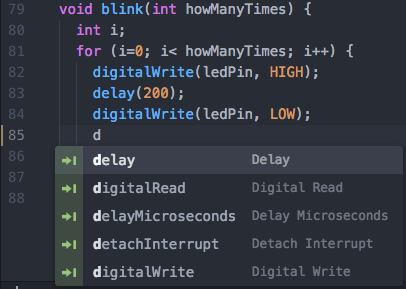
\includegraphics[width=0.43\textwidth,height=\textheight]{img/image_25.png}
\caption{Autocomplete-arduino package\label{fig:autocomplete}}
\end{figure}

Toch miste Atom een aantal belangrijke functies voor gebruik bij
robotica projecten. Zo is er geen seriële monitor (voor de tekst output
van de Arduino), geen compiler (de arduino-code omzetten in C++ code) en
is het niet mogelijk direct te builden en uploaden vanuit Atom. Dit zou
betekenen dat je eerst alle code in de Arduino IDE zou moeten plakken,
om het vanuit daar te uploaden. Gelukkig is hier een package voor,
genaamd PlatformIO. Dit voegt al deze functies, en nog veel meer, toe
aan Atom. Hier is nog een kleine toevoeging voor nodig, voor het builden
en uploaden naar de Arduino, naar de omschrijving van de ontwikkelaar
Fatsi (2015). Dit is mogelijk als de Arduino is aangesloten en de
computer hem herkent. Bij dit proces wordt de code vanaf de computer
naar de Arduino geladen.

Nu is Atom helemaal klaar voor ons project, met volledige
functionaliteit.

Om optimaal gebruik te maken van PlatformIO, moet je aan een bepaalde
folder structuur voldoen. Zo moeten er bepaalde bestanden aanwezig zijn,
en moeten bijvoorbeeld alle libraries\footnote{Bibliotheken: een
  verzameling algemene functies/routines, waardoor je geen nieuwe code
  hoeft te schrijven voor iets dat erg algemeen is of vaak voorkomt. Je
  hoeft alleen de library aan te roepen.} in de map \texttt{lib/} staan.

\hypertarget{versiebeheersysteem}{%
\subsection{Versiebeheersysteem}\label{versiebeheersysteem}}

Wij hebben alle code met behulp van een version control system (VCS)
geschreven. Hierdoor kan een van ons drieën een nieuwe functie of
verbeterde code probleemloos toevoegen. Dit kan dan herzien worden,
alvorens het vanuit een zijtak in de hoofdtak kan worden samengevoegd.
Een completere beschrijving van dit proces is te zien in
\xrefname{Fig.}\cref{fig:github}. Dit zorgt ervoor dat er niet per
ongeluk foutieve code geupload wordt, en de oudere versies dan
overschreven worden. Dit werkt bijvoorbeeld zo bij Dropbox of een andere
cloud opslag service. Door deze manier van werken is al onze broncode
ook volledig open-source, evenals alle andere bestanden die met dit
project te maken hebben. Deze zijn te vinden op onze Github pagina,
\url{https://github.com/bionicarm/bionicarm}.

\begin{figure}
\centering
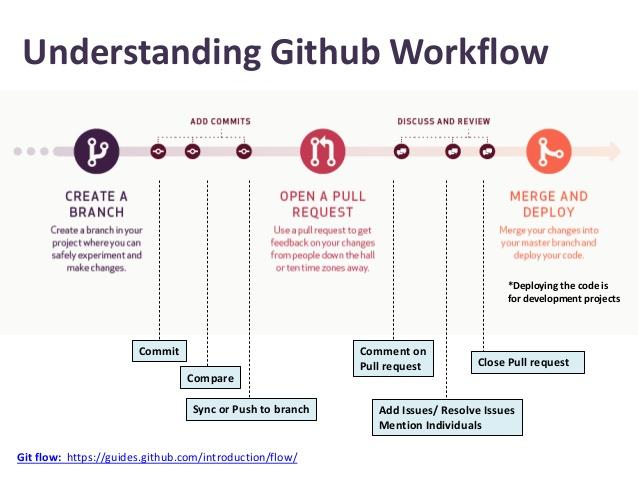
\includegraphics[width=0.65\textwidth,height=\textheight]{img/image_26.jpg}
\caption{De Github workflow, inclusief branches, commits en pull
requests\label{fig:github}}
\end{figure}

\hypertarget{toelichting-op-code}{%
\subsection{Toelichting op code}\label{toelichting-op-code}}

Bij het schrijven van arduino-code maak je altijd gebruik van twee
verplichte functies: \texttt{void\ setup()\ \{\}} en
\texttt{void\ loop()\ \{\}}. Zoals de naam misschien al verhult, gebruik
je de setup functie om alles in op te zetten en de pins hun taak te
geven. De loop functie is vervolgens het deel dat continu (in een
`loop') gaat lopen. Dit blijft net zolang doorgaan als dat er
stroomtoevoer is. Dit ziet er als volgt uit:

\begin{verbatim}
void setup() {
    // Hier plaats je alle setup-code
}

void loop() {
    // En hier alles dat uitgevoerd moet worden
}
\end{verbatim}

Voor het gebruik van servomotoren heb je de Servo bibliotheek (library)
nodig. Deze plaatsten we in \texttt{lib/Servo-master}, hierdoor konden
we in het arduino-bestand er makkelijk naar verwijzen. Daarna moeten de
motoren worden geïnitialiseerd met behulp van de library. Dit is
hieronder te zien. De structuur bij het gebruiken van een library in
Arduino is als volgt: ``Library Variabelenaam;''. Hieraan wordt
vervolgens in de \texttt{setup\{\}} functie een pinnetje aangekoppeld
met \texttt{attach()}.

\begin{verbatim}
#include <Servo.h>

Servo m1;
Servo m2;
Servo m3;
Servo m4;
Servo m5;

// SETUP
void setup() {
  m1.attach(2);
  m2.attach(3);
  m3.attach(4);
  m4.attach(5);
  m5.attach(6);
}
\end{verbatim}

Vervolgens kan de motor worden aangestuurd. Bij een servo motor doe je
dit met \texttt{m1.write(n);} waarin n een getal tussen de 0 en 180 is.
Dit komt overeen met het aantal graden die de ring op de motor draait.

Vervolgens hadden we een aantal functies om bepaalde handposities aan te
nemen. Zoals bijvoorbeeld een duim opsteken:

\begin{verbatim}
void thumbsUp() {
  m1.write(0);
  m2.write(180);
  m3.write(180);
  m4.write(180);
  m5.write(180);
}
\end{verbatim}

In deze functie staat de duim helemaal uit en de vier andere vingers
naar binnen.

De sensor moet ook worden ingesteld in de code. Dit deden wij als volgt:

\begin{verbatim}
void setup() {
  // Set EMG pin to input
  pinMode(A0, INPUT);
}

void loop() {
  // read value of analog pin 0 and give emg the value
  int emg = analogRead(A0);
}
\end{verbatim}

Om nu de handeling met de sensorwaarde te koppelen, werd er gebruik
gemaakt van een if-statement in de \texttt{loop\{\}} functie.

\begin{verbatim}
if (emg < 50) {
    allFingers(700);
} else if (emg > 50 && emg < 200) {
    pinch();
} else if (emg > 700) {
    allFingers(2300);
}
\end{verbatim}

Hier bepaald de range van de waarde voor de emg variabele welke functie
wordt uitgevoerd. In het geval dat het een bepaald getal is, wordt dat
deel van de code uitgevoerd. Zo wordt er bij emg \textgreater{} 700 de
functie \texttt{allFingers(2300)}; uitgevoerd.

De overige volledige broncode staat in de bijlage, aangevuld met kort
commentaar.
